%%
%% Beuth Hochschule für Technik --  
%%
%% Kapitel 8 - 
%%
%%	

\newpage

[Burde]
\section{Implementierung des Reglers in den realen Regelkreis}

Der kontinuierliche Regler wird nun in den realen Regelkreis implementiert. Dies wird mit Hilfe einer im PC eingebauten A/D Wandlerkarte sowie dem Realtimeworkshop realisiert. Der Regler ist dabei noch immer in einem Modell in Simulink untergebracht. Das Simulink Modell wird in Abbildung 11 dargestellt.

\begin{figure}[h]
	\begin{center}
		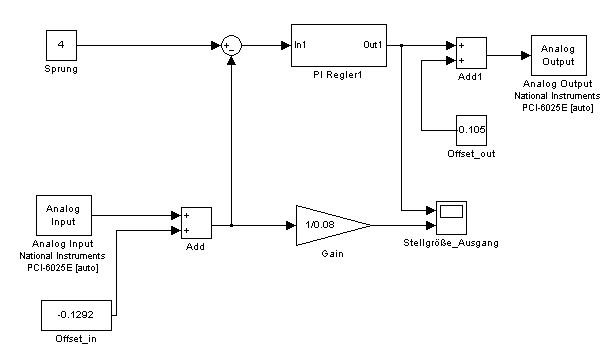
\includegraphics[scale=0.9]{modell.jpg}
		\caption{Der Regler im Simulink Modell mit Softwareschnittstellen zur A/D Wandlerkarte}
       \label{final_modell}
	\end{center} 
\end{figure}

\newpage

In der Abbildung 12 ist nun die Stellgröße und die Regelgröße des realen Regelkreises dargestellt. Die Störung wird nach ca. 6,9 Sekunden eingeschaltet und nach ca. 13 Sekunden wieder ausgeschaltet.

\begin{figure}[h]
	\begin{center}
		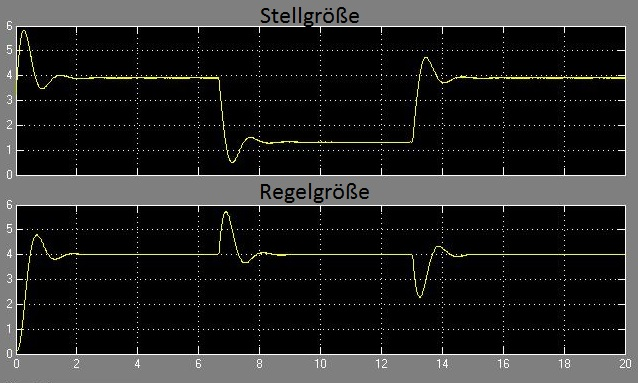
\includegraphics[scale=0.9]{scopes.jpg}
		\caption{Messungen der Regelung in der realen Strecke}
       \label{scopes_real}
	\end{center} 
\end{figure}

Aus den Diagrammen aus Abbildung 12 lassen sich einige positive Schlussfolgerungen ziehen. Der Regler regelt die Störgrößen im realen Regelkreis schnell aus, ohne dabei die Stellgröße auf über $10V$ zu übersteuern und ohne die Überschwingweite $M_{p}$ prägnant zu überschreiten. Zudem gibt es keine bleibende Regelabweichung.